%\usetikzlibrary{math}
\begin{figure}
    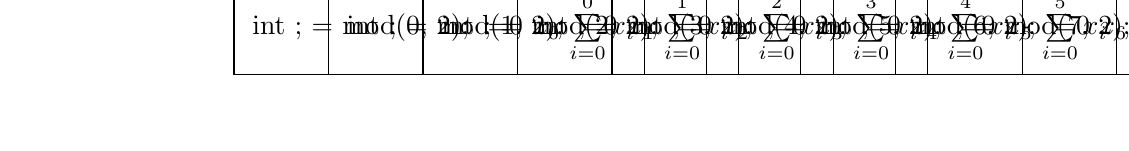
\begin{tikzpicture}[cell/.style={draw, minimum size=1.2cm}]
        \tikz\foreach \x in {0,1,...,7}
            \node[cell] at (1.2 * \x, 0) {
                %if x mod 2 == 0
                \tikzmath{
                    int \y;
                    \y = mod(\x, 2);
                }
                \ifthenelse{\y=0}
                    {$x_{\x}$}
                    {$\sum\limits_{i=0}\limits^{\x} x_i $}
            };
    \end{tikzpicture}
    \caption{Prefix Sum Upsweep}
    \label{fig:prefix_sum_upsweep}
\end{figure}